%% grundlagen.tex
%% $Id: grundlagen.tex 28 2007-01-18 16:31:32Z bless $
%%

\chapter{Grundlagen \& aktuelle Forschung}
\label{ch:Basics}

\section{Schlafmedizin}
\label{ch:Basics:se:schlafmedizin}
% start seite 3-5 im buch schlafmedizin_1x1 
Unter dem Begriff \textit{Schlafmedizin} versteht man die Lehre von Diagnostik, Klassifikation und Behandlung von Störungen während des Schlafs \cite{croenleinSchlafmedizin1x1Praxisorientiertes2017}. 
Trotz Erwähnungen in der Antike gewinnt Schlafmedizin erst seit dem letzten Jahrhundert an Bedeutung.
Mithilfe der Polysomnographie konnten unterschiedliche Schlafphasen zyklischen Ablaufs erkannt werden.
Zudem konnten zu den Schlafphasen physiologische Eigenschaften nachgewiesen werden.
Heutzutage sind ca. 80 Schlafstörungen in dieversen Bereichen bekannt, welche neben psychologischen Testverfahren überwiegend elektrophysiologisch untersucht und behandelt werden.
Patienten werden mit ambulanten Hilfsmitteln oder stationär in einem Schlaflabor untersucht und diese dabei ermittelten Daten werden anschließend von einem technisch ausgebildeten Personal analysiert.

Hierbei wird eine Polysomnographie durchgeführt, womit genauere Messergebnisse im Vergleich zu einem ambulanten Hilfsmittel (z.B eine Langzeitbewegungsmessung) erreicht werden können.
Während einer Polysomnographie werden Gehirnströme, Augenbewegungen und Muskelspannungen erkannt, wodurch die einzelnen Schlafphasen unterschieden werden können.
Die verschiedenen Sensorwerte werden dann in Form eines Hypnogramms mittels der Kriterien des AASM (engl. \textit{American Association for Sleep Medicine}) ausgewertet (siehe Abbildung \ref{hypnogram_example}). 
Hierbei werden die Schlafstadien in \textit{Wachphase (w)}, \textit{Einschlafen (N1)}, \textit{leichten Schlaf (N2)}, \textit{Tiefschlaf (N3)} und \textit{Rapid-Eye-Movement-Schlaf (REM)} unterteilt.

\begin{figure}[ht]
    \centering
    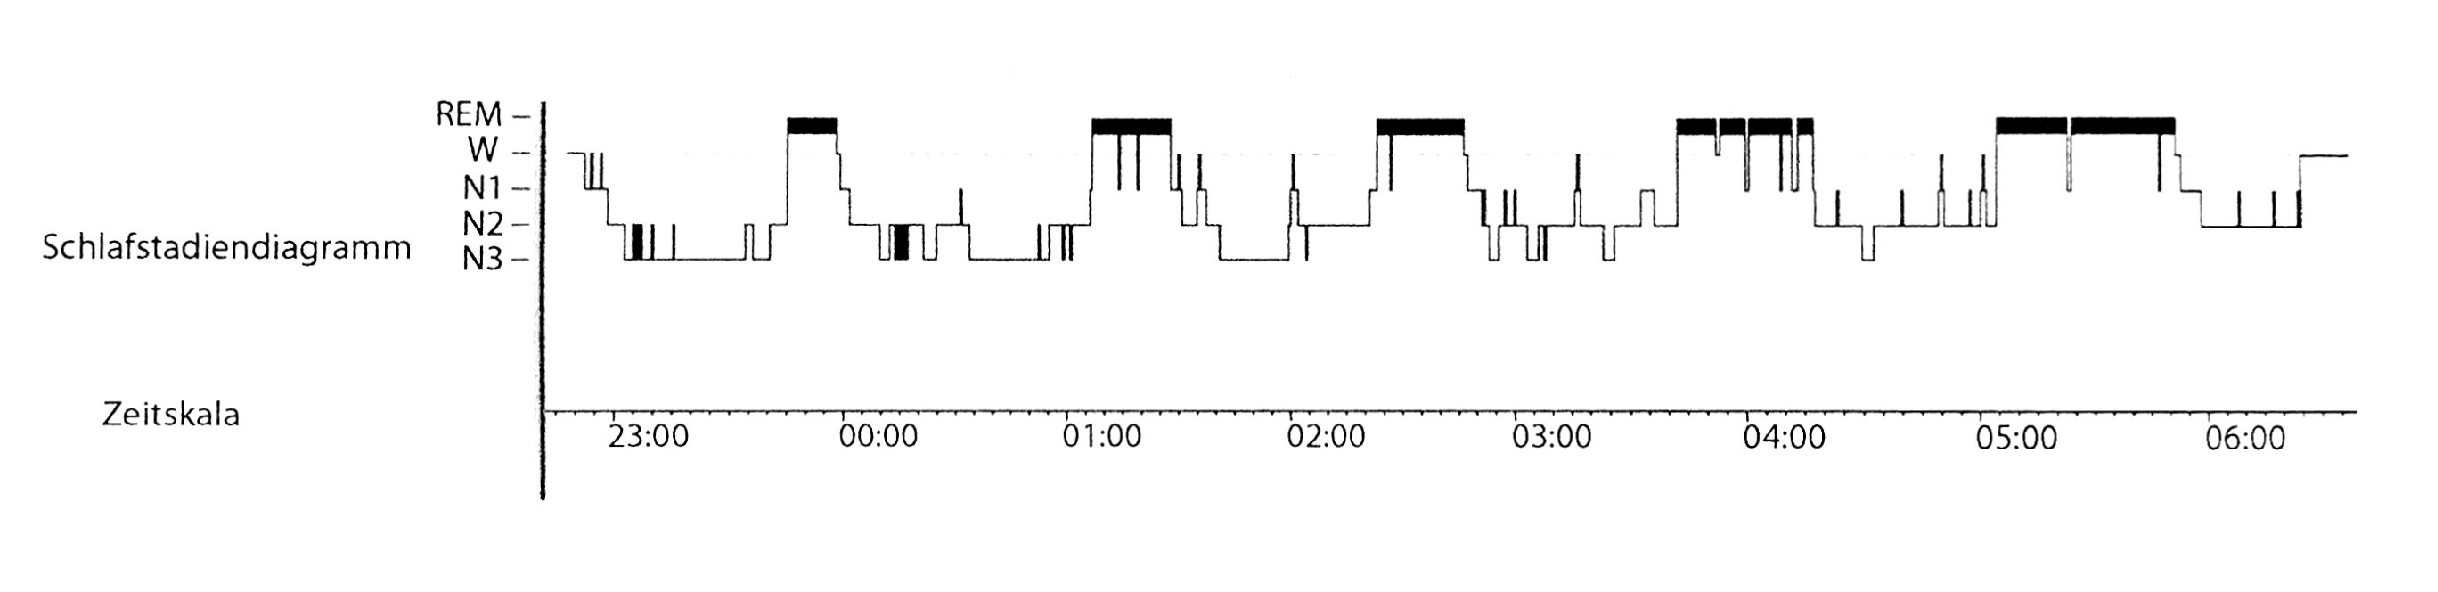
\includegraphics[scale=0.33]{respiration/hypnogram_example}
    \caption{Beispielaufzeichnung, dargestellt in einem Hypnogramm \cite{stuckPraxisSchlafmedizinDiagnostik2018}}
    \label{hypnogram_example}
\end{figure}

% ende cite
% start seite 9- im buch schlafmedizin_1x1 
Im Schlaflabor werden zudem auch Untersuchungen der Müdigkeit, der Tagesschläfrigkeit und der Aufmerksamkeit vorgenommen \cite{croenleinSchlafmedizin1x1Praxisorientiertes2017}.

Atmungsstörungen können oft die Ursache von Schlaganfällen, Herzinfarkten oder den eben genannten Symptomen sein, welche zu erheblichen psychischen Störungen führen können.
% ende cite
Aus diesem Grund ist es wichtig, so genau wie möglich Schlafstörungen bestimmen zu können, um Folgeerkrankungen zu verhindern. 

\section{Klassifizierung von Schlafstörungen}
\label{ch:Basics:se:classification}
Zur Charakterisierung von Schlafstörungen werden viele Biosignale während des Schlafs registriert, die entscheidene Merkmale liefern \cite{stuckPraxisSchlafmedizinDiagnostik2018}.
Aufgrund dieser Annahme wurde eine Einteilung in 7 Klassifikatoren für Schlafstörungen entwickelt.
\begin{itemize}
    \item Ein- und Durchschlafstörungen (Insomnien)
    \item schlafbezogene Atmungsstörungen
    \item Hypersomnien zentralnervösen Ursprungs
    \item zirkadiane Rhythmusschlafwachstörungen
    \item Störungen in Verbindung mit Schlaf, Schlafstadien oder partiellem Erwachen (Parasomnien)
    \item schlafbezogene Bewegungsstörungen
    \item andere Schlafstörungen
\end{itemize}

Diese Gliederung orientiert sich an der \textit{ICSD-3} \cite{stuckPraxisSchlafmedizinDiagnostik2018}.


Diese Bachelorarbeit is darauf fokussiert, eine zentrale Schlafapnoe zu klassifizieren, die Bestandteil der {\glqq schlafbezogenen Atmungsstörungen\grqq} ist.
Neben der zentralen Apnoe gibt es die obstruktive Apnoe. 
Hierbei sind die Atemwege geschlossen und eine Atmung ist für mehrere Sekunden unmöglich.
Circa 20\% aller Erwachsenen haben fünf oder mehr obstruktive Ereignisse pro Schlafstunde \cite{croenleinSchlafmedizin1x1Praxisorientiertes2017}.
Zentrale Apnoe hingegen tritt seltener auf, als obstruktive Apnoe, jedoch auffällig oft bei besonderen Patientengruppen. 
Ein Beispiel liefern Patienten mit Herzinsuffizien und einer eingeschränkten kardialen Pumpfunktion.
72\% dieser Patientengruppe leiden unter einer zentralen Schlafapnoe. 
Dies macht die Bedeutung der Klassifikation deutlich, da eine genaue Erkennung einer zentralen Apnoe hier sehr wichtig ist.

\subsection{Zentrales Schlafapnoe}
\label{ch:Basics:se:apnoe}
Bei der zentralen Apnoe steht der Luftfluss trotz offener Atemwege für mindestens $10\si{\s}$ still. 
Dies kann vollständig (zentrale Apnoe), oder partiell (zentrale Hypopnoe) erfolgen. 
Ab einer Anzahl von fünf Apnoeereignissen wird zentrale Apnoe diagnostiziert.
Die Ursachen gelten hierbei als internistische oder neurologische Grundlage.
Typische an- und abschwellige Muster sind auf eine chronische Herzinsuffizienz, auf eine verlängerte Kreislaufzeit, oder durch eine zentralnervöse Verstellung der sogenannten Apnoeschwelle zurückzuführen.
Der $CO_2$ Gehalt im Blut wird als Apnoeschwelle bezeichnet.
Am Tag sind die Symptome von zentralem Apnoe eher an deren Ursache, den internistischen und neurologischen Grunderkrankungen zu erkennen, da diese häufig nicht von den Symptomen der Schlafapnoe zu unterscheiden sind. 
In der Nacht wird zentrales Apnoe, ebenso wie obstruktives Apnoe an Atemaussetzern, häufig vom Partner des Patienten beobachtet.
Zudem kann lautes und unregelmäßiges Schnarchen ein Indiz für ein Apnoe sein, ebenso wie ein Aufwachen in Atemnot.

Ein Schlafapnoe kann jedoch in unterschiedlichen Schweregraden auftreten. 
Es gibt Patienten, welche kaum bis keine Probleme haben und nur aufgrund von nächtlichen Erkenntnissen ihrer Ehepartner zum Arzt geschickt werden. 
Es gibt jedoch auch Patienten, die am Tag Probleme haben, bei monotonen Situationen wach zu bleiben.

Eine Diagnose würde mögliche Folgeerkrankungen schneller erkennbar machen und die Ursache dieser erklären.

\section{Maschinelle Lernverfahren}
\label{ch:Basics:se:ml}
Zur Klassifikation eines zentralen Apnoes werden im Rahmen dieser Bachelorarbeit verschiedene Klassifikationsverfahren verwendet, wobei Trainingsdaten gesammelt werden, welche dann zentrale Apnoeereignisse anhand dieser Trainingsdaten klassifizieren sollen.

Maschinelle Lernverfahren sind Algorithmen, welche die Performance des Algorithmus mittels Trainingsdaten verbessern \cite{neumannMaschineLearningKIT2020}. 
Es wird zwischen folgenden Lernverfahren unterschieden:
\begin{itemize}
    \item Supervised Learning
    \item Unsupervised Learning
    \item Reinforcement Learning
\end{itemize}
Beim \textit{Supervised Learning} sind die Trainingsdaten im Vergleich zum \textit{Unsupervised Learning} markiert und anhand dessen wird eine Entscheidung getroffen. 
Die folgenden Tabelle zeigt die Unterschiede der verschiedenen Modelle bei \textit{Supervised} und \textit{Unsupervised Learning}:
\begin{center}
    \begin{tabular}{ | l | l | }
      \hline
      \textbf{Supervised Learning} & \textbf{Unsupervised Learning} \\ \hline
      \hline
      Regression & Clustering \\ \hline
      Klassifikation & Dimensionsreduktion \\
      \hline
    \end{tabular}
\end{center}

Jeder Algorithmus, welcher in einem dieser Modelle des Maschinellen Lernverfahrens eingesetzt ist, besteht aus 3 Teilen: Zum einen der \textit{Representation}, der \textit{Evaluation} und der \textit{Optimization}. 
In der \textit{Representation} unterscheidet man nach dem zugrunde liegenden Modell, welches beispielsweise ein Entscheidungsbaum, ein neuronales Netz oder eine Support-Vektor-Maschine sein kann.
Die \textit{Evaluation} behandelt die Frage, in welche Richtung die Entscheidung getroffen werden soll. 
Ein Beispiel hierfür wäre die Genauigkeit, den Precision \& Recall, die Entropie oder den Likelihood-Schätzer.
Beim dritte Teil, der \textit{Optimization}, wird eine Optimierung des Algorithmus angestrebt. 
Dies kann unter anderem mit Methoden zweiter. Ordnung, zufälliger Suche, einem absteigenden Gradienten oder der Methode der kleinsten Quadrate versucht werden.

Das in dieser Bachelorarbeit verwendete Lernverfahren ist \textit{Supervised Learning} mit dem zugehörigen Modell, die \textit{Klassifikation}.
Zur Evaluation wurden verschiedene Klassifkationsverfahren verwendet, welche im Folgenden genauer erläutert werden.

\subsection{Random Forest}
\label{ch:Basics:se:ml:ss:randomForest}

Random Forest ist ein Klassifikationsverfahren des \textit{Supervised Learning} \cite{WaybackMachine2016}. 
Zur Klassifikation werden markierte Daten vorausgesetzt, woraus eine gelernt mathematische Representation erstellt wird (\textit{model}). 
Dieses Modell wird anschließend genutzt, um auf unmarkierten Daten eine Vorhersage zu treffen.
Random Forest basiert auf Entscheidungsbäumen. 
Das sind Bäume, bei welchen pro Ast eine Entscheidung getroffen wird.
Sie lernen binäre Entscheidungsregeln, die einer logischen Abfolge entsprechen.
Jedoch sind einzelne Entscheidungsbäume nicht robust genug und neigen zu Overfitting.
Random Forest nutzt deshalb viele Entscheidungsbäume und trainiert auf dem selben Trainingsdatensatz. 
Der Zusammenschluss der Entscheidungen jedes Entscheidungsbaums repräsentiert die endgültige Entscheidung.
Bei Random Forest werden bei jeder Verästelung eine zufällige Teilmenge der Features in Betracht gezogen, was den Einfluss von stark korrellierenden Features verringern soll.

Entscheidungsbäume können allgemein durch verschiedene Arten zusammengetragen werden. 
Zum einen ist dies mit \textit{Bagging}, zum anderen mit \textit{Boosting} möglich.
Bei \textit{Bagging} werden zufällige Stichproben aus der Datenmenge für jeden Entscheidungsbaum genommen \cite{jamesIntroductionStatisticalLearning2013}.
Je nach Wahl geschieht dies mit oder ohne Zurücklegen dieser zufälligen Teilmenge für den nächsten Entscheidungsbaum.
Bei Bagging werden die Entscheidungsbäume parallel trainiert, was sich positiv auf die Performance auswirkt.
Bei \textit{Boosting} werden ebenfalls Teilmengen pro Entscheidungsbaum aus der Datenmenge gepickt, jedoch nicht zufällig. 
Es werden schwierige Fälle höher gewichtet, wodurch diese häufiger in einen Entscheidungsbaum mit aufgenommen werden. 
Somit werden die darauffolgenden Entscheidungsbäume mit Zurücklegen der Teilmenge ausgewählt.
Falls eine falsche Vorhersage auf einen Datenbestand getroffen wurde, erhöht sich die Gewichtung.
Die Wahrscheinlichkeit ist nun höher, dass dieser Datenbestand im nächsten Entscheidungsbaum enthalten ist.
Die Entscheidungsbäume werden bei Boosting sequenziell trainiert.

Random Forest verwendet \textit{Bagging}. 
Die endgültige Entscheidung ist entweder ein Mehrheitsvotum oder der Durchschnitt der Vorhersagen aller Trainingsläufe.
Bei Random Forest können zusätzlich einige Hyperparameter modifiziert werden, wie unter anderem die Anzahl der zu kombinierenden Entscheidungsbäume, die maximale Baumtiefe oder die maximalen Features pro Verästelung. 
Die Vorteile von Random Forest sind die Schnelligkeit, die Flexibilität und die Parallelisierbarkeit.
Zudem gibt das Resultat nicht nur die entgültige Entscheidung, sondern die Wahrscheinlichkeit der Entscheidung, an.
Zu den Nachteilen zählt die schlechte Performance bei seltenen Klassen und die Anfälligkeit für Overfitting.
Des weiteren ist Random Forest ein Blackbox Modell, wodurch es kaum möglich ist, zu ermitteln, wie die Entscheidung getroffen wurde.

\subsection{XGBoost}
\label{ch:Basics:se:ml:ss:xgboost}
Bevor XGboost erklärbar ist, muss \textit{Gradient Boosting} eingeführt werden.
Gradient Boosting ist wie Random Forest ein Teil des Überwachten Lernens (\textit{Supervised Learning}) und kann für die Klassifikation oder Regression verwendet werden \cite{friedmannStochasticGradientBoosting1999}. 
Zudem ist Gradient Boosting wie Random Forest ein Emsemble-Learner, d.h. sie setzen sich aus vielen einzelnen Modellen (den Entscheidungsbäumen) zusammen.
Im Gegensatz zu Random Forest verwendet Gradient Boosting nicht Bagging, sondern \textit{Boosting}.
Wie schon im Kapitel \ref{ch:Basics:se:ml:ss:randomForest} eingeführt, trainiert \textit{Boosting} zufällig gewichtete Stichproben aus einer Datenmenge mit Zurücklegen. 
Falsche Entscheidungen erhöhen die Gewichtung, richtige Entscheidungen verringern die Gewichtung jeder Vorhersage. 
Somit werden schwierige Fälle besonders beachtet, da die Anpassung der Gewichtungen nach jeder Vorhersage stattfindet, also bevor die neue Teilmenge anhand der Gewichtung bestimmt wird.
Das Trainieren auf Teilmengen wird auch als stochastisches Gradient Boosting bezeichnet und verringert die Wahrscheinlichkeit auf Overfitting.
Zudem wird eine bessere Generalisierbarkeit erreicht.

Zu Beginn wird ein Basismodell, bestehend aus den Entscheidungsbäumen gewählt, worauf anschließend Vorhersagen anhand der Trainingsdaten getroffen werden. 
Daraufhin werden die Gewichte angepasst, je nach der getroffenen Vorhersage. 
Aus dem Basismodell mit den nun angepassten Gewichten wird eine Teilmenge gewählt, womit erneut Entscheidungsbäume entstehen und Vorhersagen getroffen werden können.
Bei Gradient Boosting wird nun mittels Gradienten der Fehler der verschiedenen Emsembles minimiert.
Auch hier gibt es Hyperparameter, welche angepasst werden können. Diese sind sehr ähnlich zu Random Forest, werden jedoch um diverse Parameter erweitert, wie zum Beispiel der Funktion, welche den Fehler berechnet, die Anzahl der Iterationen pro Baum oder auch die Anzahl der Instanzen pro Blatt.

XGboost ist nun eine spezielle Version des Gradient Boosting, und zwar das \textit{Extreme Gradient Boosting} \cite{chenXGBoostScalableTree2016}.
Der Unterschied zu Gradient Boosting ist hierbei, dass bei der Fehlerfunktion (Loss-Funktion) die Gradienten 2. Ordnung gewählt werden, wodurch mehr Informationen für die Verringerung des Fehlers bereit stehen.
Zudem können dadurch die besten Entscheidungsbäume approximiert werden. 
XGBoost verwendet außerdem L1 \& L2 Regularisierung, dadurch kann besser generalisiert werden und Overfitting vermieden werden.
XGBoost ist parallelisierbar, schnell und kann zudem für verteiltes Trainieren auf Clustern betrieben werden.

\subsection{Support Vektor Maschine (SVM)}
\label{ch:Basics:se:ml:ss:svm}
Eine Support Vektor Maschine ist ein Klassifikationsverfahren für Probleme, welche in zwei Klassen gruppiert werden \cite{cortesSupportvectorNetworks1995}.
Bei der linearen Support Vektor Maschine wird nun eine {\glqq Trennlinie\grqq} gesucht, welche die Menge der Daten in 2 Klassen gruppiert. 
Diese Trennlinie wird optimiert.
Es gibt auch eine nichtlineare SVM, die eine nichtlineare Trennlinie sucht.
Hierbei kann es jedoch zu Overfitting kommen, da eine nichtlineare Trennlinie durch potenzielle Outlier sehr komplex werden kann und zu {\glqq gut\grqq} optimiert wird.
Jeder Wert im Datensatz ist ein Support Vektor und somit ein repräsentativer Punkt, welcher bei der Klassifikation gruppiert werden soll.
Die Trennlinie muss also zwischen allen markierten Daten unterscheiden können.
Jedoch ist die Komplexität hierbei sehr hoch, da eine Trennlinie, beziehungsweise eine Trennebene im hochdimensionalen Raum nur mit sehr hohem Aufwand gefunden werden kann.
Die Suche nach der Trennline kann durch mehrere Kernel verschieden bestimmt werden.
Die beliebtesten Kerneltypen sind:

\begin{center}
    \begin{tabular}{ | l | c | r | }
        \hline
        Kernel Name & Kernel Funktion \\ \hline
        Linear Kernel & $K(x)=x \cdot y$ \\ 
        Polynomial Kernel & $K(x)=(x\cdot y+1)^d$ \\
        Radial Basis Function (RBF) Kernel & $K(x)=e^{-\gamma(\Vert x-y \Vert)^2}$ \\
        \hline
    \end{tabular}
\end{center}

Die korrekte Wahl des richtigen Kernels ist entscheidend für deren Performance und Genauigkeit, jedoch nicht so leicht zu wählen.
Die Vorteile von SVM sind die Effektivität im hochdimensionalen Raum, des weiteren ist SVM speichereffizient und zudem können durch die verschiedenen Kerneltypen mehrere Datensätze variabler verarbeitet werden.
Zu den Nachteilen zählt, dass Performance schlecht ist, wenn die Anzahl der Features größer als die Anzahl der Samples ist. 
Zudem neigt SVM gerade im nichtlinearen Bereich schnell zu Overfitting.

\section{Forschung von Klassifikation anhand von IMU-Daten}
Es gibt bereits Ansätze, welche sich damit befassen, Alternativen zur Ermittlung von Schlafstörungen zu finden. 
Somit könnte ein Besuch im Schlaflabor durch einen bequemen Test ersetzt werden. 
Ein vielversprechender Ansatz ist es, mittels IMU-Daten die Bewegung des Körpers zu messen und anhand dieser Informationen unter anderem die Atmung herauszufiltern, um dann Rückschlüsse auf Schlafstörungen schließen zu können.

\subsection{Beschleunigungssensor am Brustkorb}
Bereits 2018 gab es Forschung in diesem Bereich. \textit{Phan Duy Hung} hat sich damit befasst, einen Beschleunigungssensor (\textit{Accelerometer}) an den Brustkorb zu fixieren \cite{hungCentralSleepApnea2018}.
Durch die Platzierung an genau dieser Stelle wurde der Herzschlag genauer erkannt. 
Die Rohdaten zeigen hierbei bereits die Herzfrequenz und die Atmung des Probanden (siehe Abb. \ref{imu_research_hung_rawData}). 

\begin{figure}[ht]
    \centering
    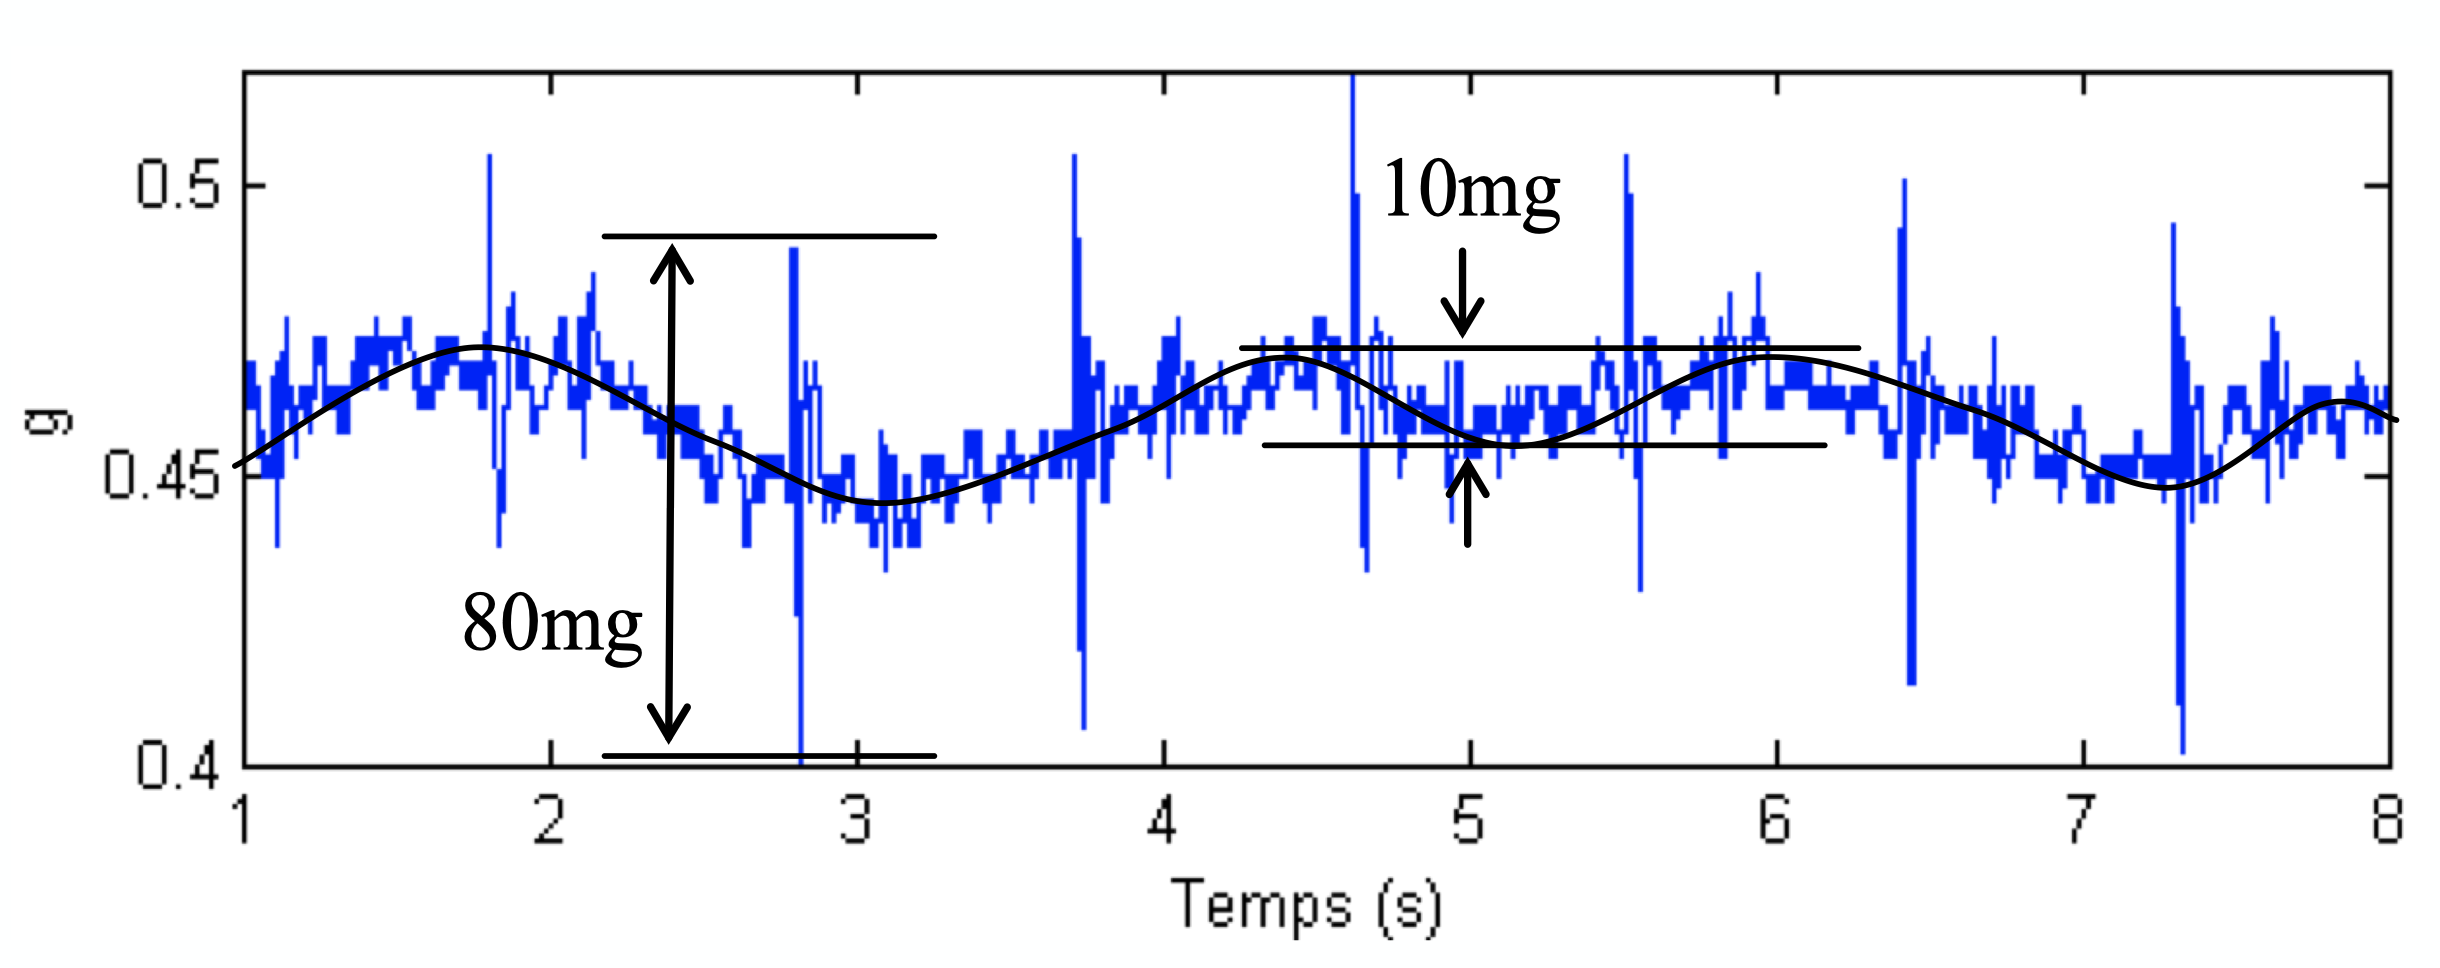
\includegraphics[width=1\textwidth]{imu_research/Paper_Hung_rawData}
    \caption{Rohdaten des Accelerometers in \cite{hungCentralSleepApnea2018}}
    \label{imu_research_hung_rawData}
\end{figure}

Die Daten wurden nach der Aufzeichnung durch einen Bandpassfilter mit adaptiver Apassung optimiert, um die SNR (\textit{signal-noise-ratio}) zu verringern.
Der Puls wurde ermittelt, indem Peaks (Max: \textit{V}-Peak, Min: \textit{R}-Peak) gefunden und als Herzschlag interpretiert wurden.
Des weiteren musste Signalrauschen, z.B von der Reibung des T-Shirts und der Haut, aus dem Signal herausgefiltert werden. 
Zudem wurden 3 Features anhand der Amplitude über die Zeit berechnet. 
Das erste Feature ist das \textit{Spektralverhältnis (spectral ratio)}. 
Hier wird ein Leistungsspektrum eines einminütigen Segments vom HR-Signal geschätzt. 
Der Frequenzbreich zwischen [0-1] $\si{\hertz}$ wurde untersucht. 
Dieser Bereich spiegelt die Frequenzvariation zwischen zentraler Schlafapnoe und normaler Aktivität wieder.

Im Bereich von [0,3-0,6] Hz zeigt sich das Maximum der spektralen Leistung, was immer in der Größenordnung abnimmt. 
Dieser Wert wird normiert, indem er durch den Mittelwert der spektralen Leistung im Bereich [0,1-0,3] Hz geteilt wird. 
Das Verhältnis der max(P) im Bereich von [0,3-0,6] Hz zum Mittelwert(P) in [0,1-0,3] Hz ist unabhängig von der Person.

Das zweite Feature sind die \textit{Wavelet- Koeffizienten (wavelet coefficients)}, bei welcher die Analyse mit mehreren Auflösungen und guter Lokalisierungsfähigkeit im Zeit-Frequenz-Bereich häufig als eine Wavelet-Transformation verwendet wird. 
Hierbei wurde das Atemsignal in 5 Ebenen mit der db2-Wavelet zerlegt. Danach wurden die Standardabweichungen der Detailkoeffizienten in den Ebenen 4 und 5 verwendet. 

Das dritte Feature sind die \textit{linear prediction coefficients}. 
Die zweite Ordnung der linearen Vorhersage
\begin{center}
    $x(n) = a_1 x(n-1) + a_2 x(n-2) + e(n)$
\end{center} 
wurde verwendet, wobei x eine Zeitreihe ist, e(n) der Vorhersagefehler und {a1, a2} die Vorhersagekoeffizienten, die durch die Least-Square-Optimierungsverfahren zu bestimmen sind.

Die folgenden Werte wurden zum Testen mit ANOVA ausgewählt: \\
ANOVA: $a_1$, $a_2$ und $\sqrt{a_1^{2} + a_2^{2}}$


Zudem wurden nichtlineare Features in Betracht gezogen, da bereits vorher festgestellt wurde, dass in komplexen Atemuntersuchungen lineare Funktionen nicht ausreichen. Die Herzfrequenz wird hierbei als Timeseries betrachtet.
Es wurden diesbezüglich die nichtfunktionalen Features der \textit{Poincaré-Plots (Poincare plot geometry)}, \textit{Trendbereinigende Fluktuationsanalyse (Detrended Fluctuation Analysis)}, \textit{Approximate-Entropie (Approximate Entropy)}, sowie der \textit{Ljapunow-Exponent (Largest Lyapunov exponent)} verarbeitet. 

Die Features wurden anschließend mit der \textit{ANOVA-Toolbox} ausgewertet.
Somit konnte ermittelt werden, ob in dem zeitlichen Intervall eine Apnoe stattgefunden hat, oder nicht.

Durch dieses Paper wurde eine Genauigkeit von 84.2\% erreicht.
Eine zentrales Apnoe ließ sich zu 84.1\% erkennen, woraus ermittelt werden konnte, dass in diesem Zeitrahmen keine zentrale Apnoe vorkam.


\subsection{Detektion direkt am Kopf mittels der Google-Glass Brille}
2015 wurde bereits erforscht, durch Informationen des Google-Glass den Puls und das Atemsignal zu ermitteln \cite{hernandezCardiacRespiratoryParameter}. 
Der Vorteil hierbei ist die Position der Brille. 
Da sie am Kopf platziert ist, liefert die Brille möglicherweise vielversprechende Werte im Vergleich zu IMU-Daten, die am Brustkorb aufgezeichnet worden sind.
Die Google-Glass Brille wurde allerdings nicht entwickelt, um physiologische Daten zu sammeln, kann jedoch dafür verwendet werden, da alle nötigen Sensoren (Accelerometer, Gyroscope und Kamera) darin verbaut sind.
Die Resultate liefern einen mittleren absoluten Fehler (\textit{MAE}) von 0.82 Schlägen pro Minute (STD: 1.98) der Herzrate und 0.6 Atmungen pro Minute (STD: 1.19) bei der Atmung unter Betrachtung verschiedener Beobachtungsfenster und Kombinationen der Sensoren. 
\begin{figure}[ht]
    \centering
    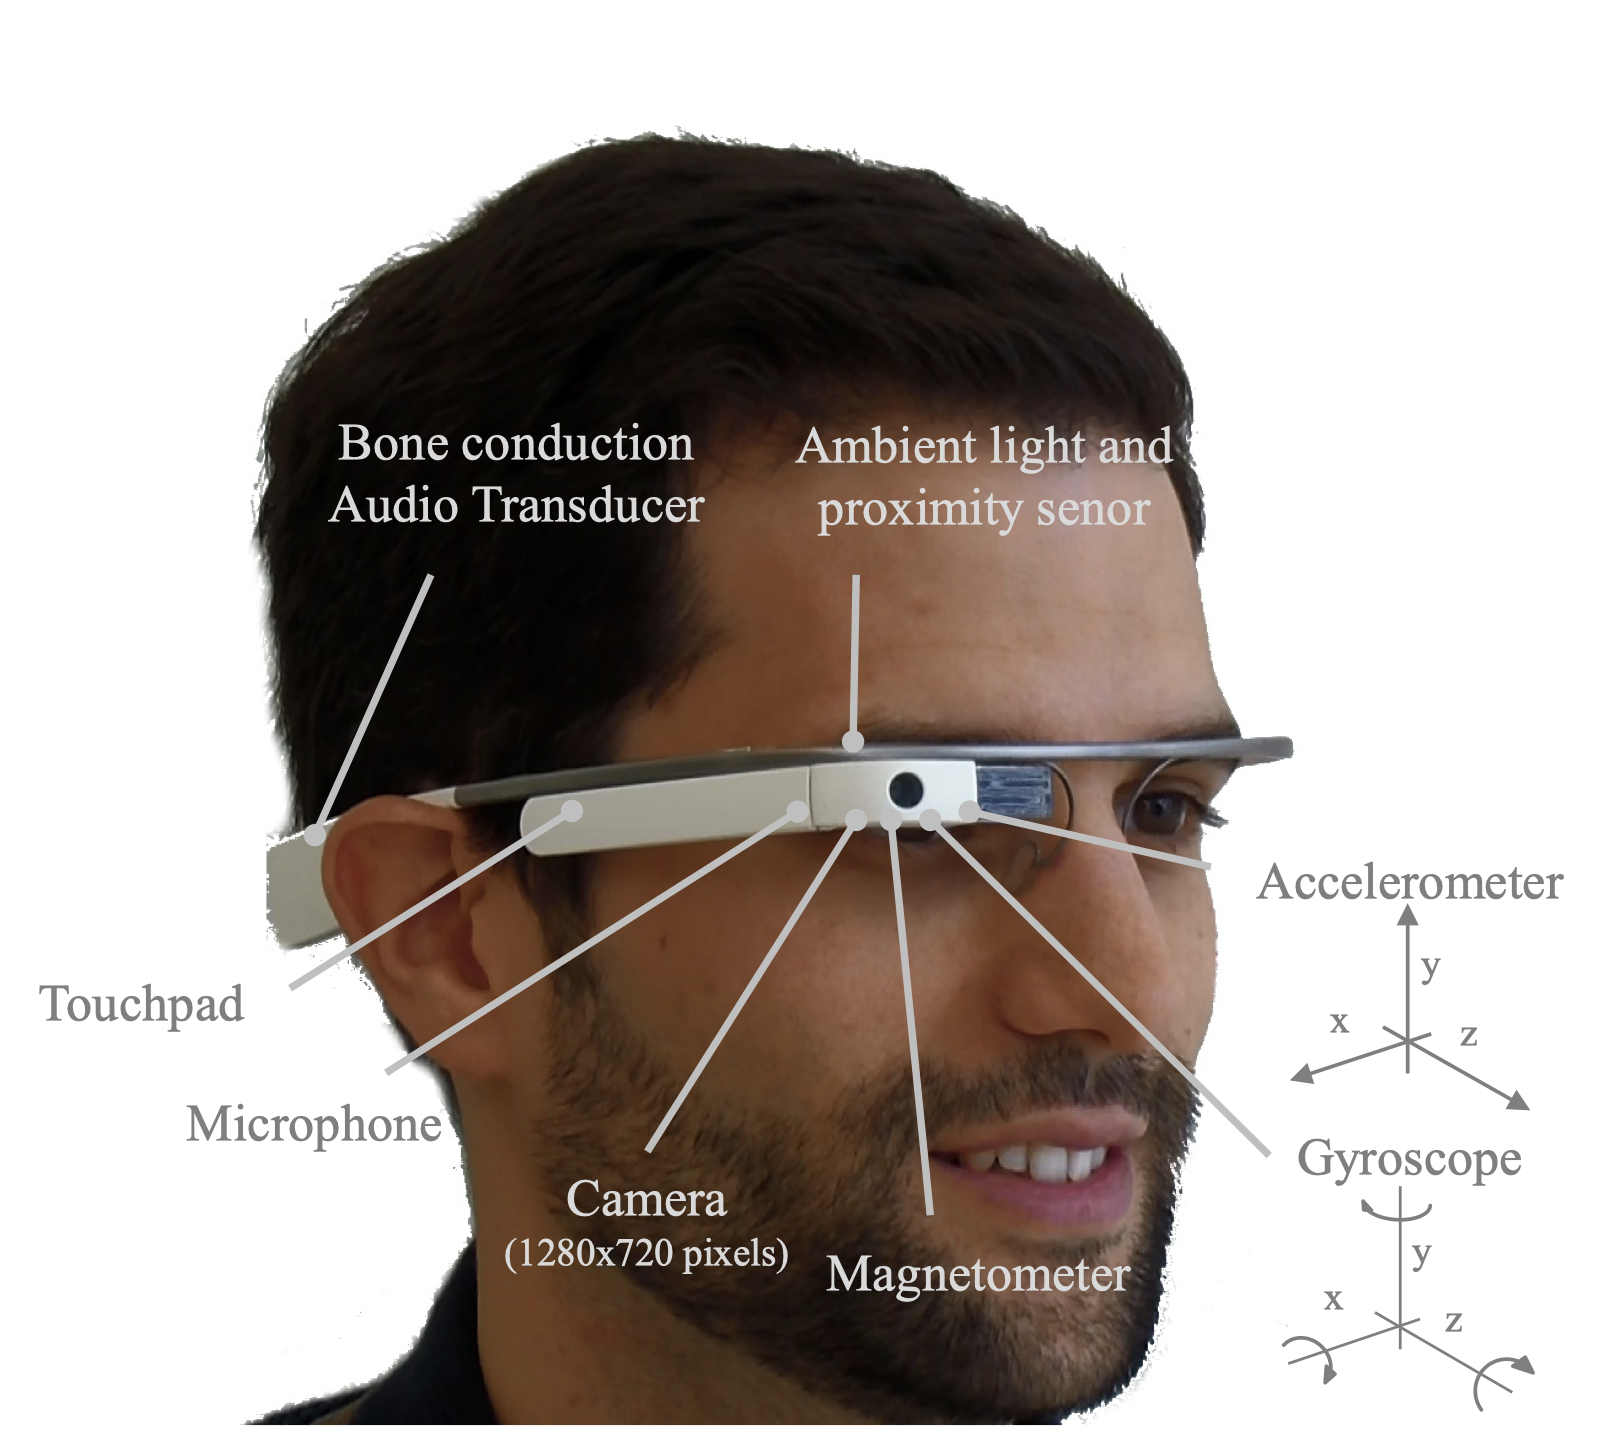
\includegraphics[width=\textwidth / 2]{imu_research/googleGlass}
    \caption{Google Glass Sensordaten \cite{hernandezCardiacRespiratoryParameter}}
    \label{imu_research_google_glass}
\end{figure}
Die Herausforderung lag zudem daran, stromsparende Echtzeitberechnungen mit Algorithmen zu entwickeln, womit physiologische Parameter extrahiert werden. Der Nutzer soll das Gerät im Alltag normal weiternutzen können. 

Es wurden 2 Techniken entwickelt, eine zur Ermittlung des Pulssignals, die andere für das Atemsignal.
\subsubsection{Pulssignal}
Die Schätzung des Pulssignals wurde anhand einer Timeseries von Vektoren in mehrere Schritte aufgeteilt:
\begin{itemize}
    \item Von jeder Dimension des Vektors wurde ein gleitendes Durchschnittsfenster von 3 Abtastwerten subtrahiert, wodurch Signalverschiebungen und Trends entfernt werden konnten.
    \item Ein Bandpass Butterworthfilter der 4. Ordnung mit den Cut-Off Frequenzen von $10 \si{\hertz}$ und $13 \si{\hertz}$ wurde auf jede Dimension angewandt, um Veränderungen des BCG zu isolieren.
    \item Zudem wurde ein Bandpass Butterworthfilter der 2. Ordnung mit den Cut-Off Frequenzen von $0.75 \si{\hertz}$ und $2.5 \si{\hertz}$ (entspricht 45 and 150 Schläge die Minute) angewandt, was schließlich das resultierende Pulssignal liefert.
\end{itemize}

\begin{figure}[ht]
    \centering
    \begin{subfigure}{.49\textwidth}
        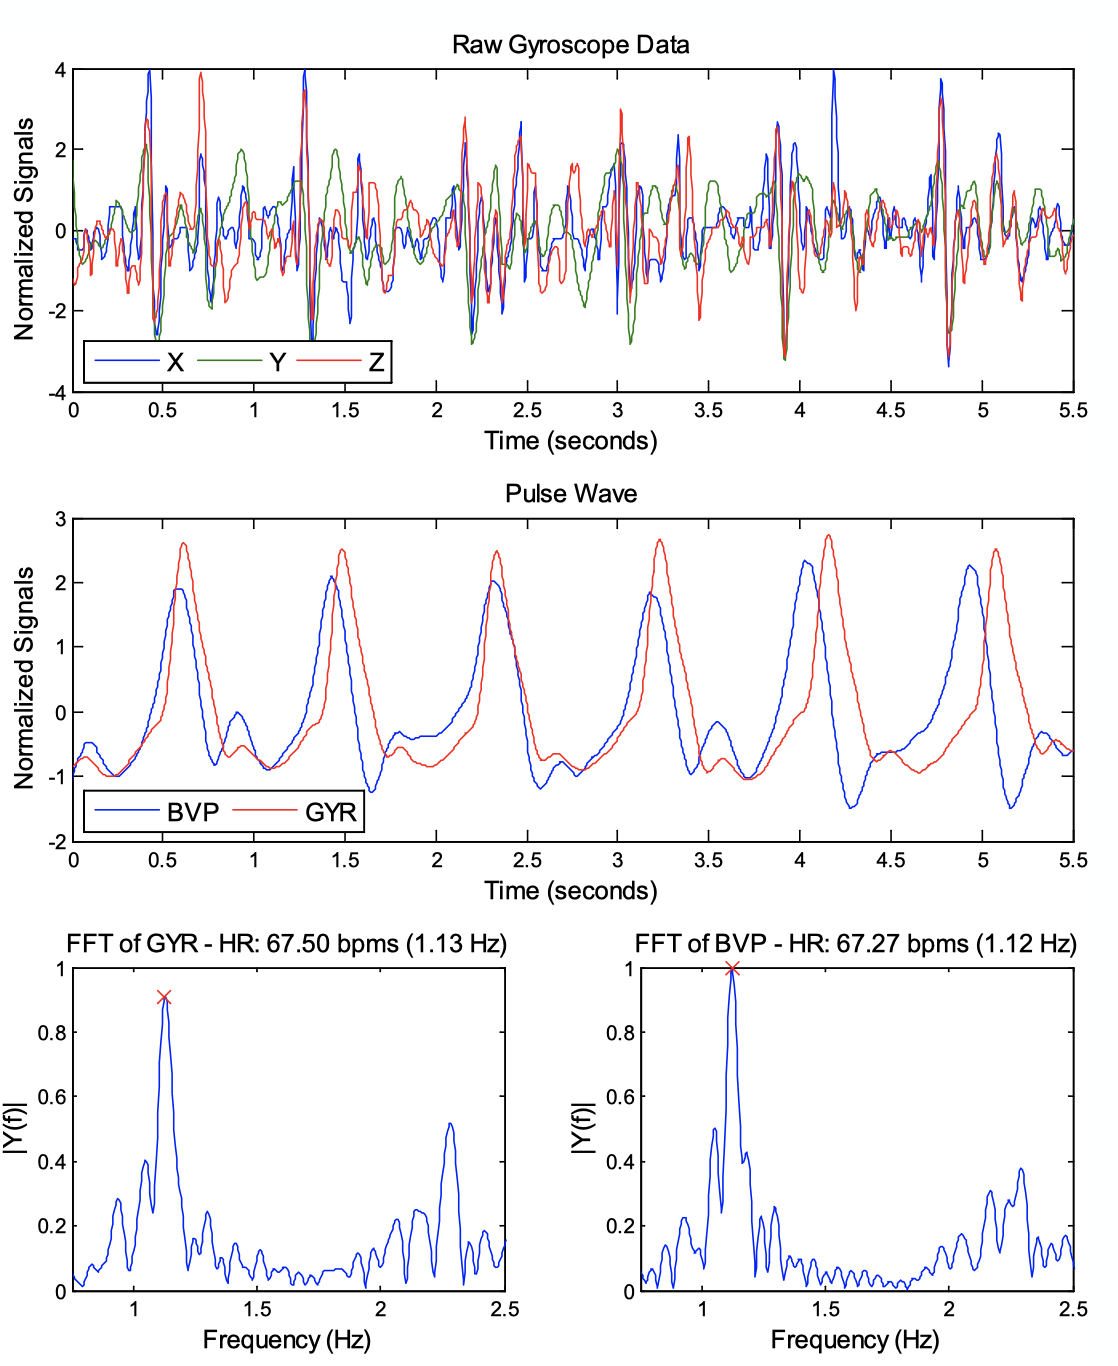
\includegraphics[width=\textwidth]{imu_research/googleGlass_pulse_fig2}
      \caption{Beispiel eines Pulssignals mittels der Gyroskopdaten (rot) und des Ground-Truth Signals (blau). Die beiden unteren Graphen zeigen das Fouriespektrum von jedem Signal (FFT: Fourier Spectrum, GYR: Gyroscope, BVP: Blood Volume Pulse, HR: Heart Rate, bpms: beats per minute)}
      \label{background:googleGlass:pulse_wave}
    \end{subfigure}
    \begin{subfigure}{.49\textwidth}
        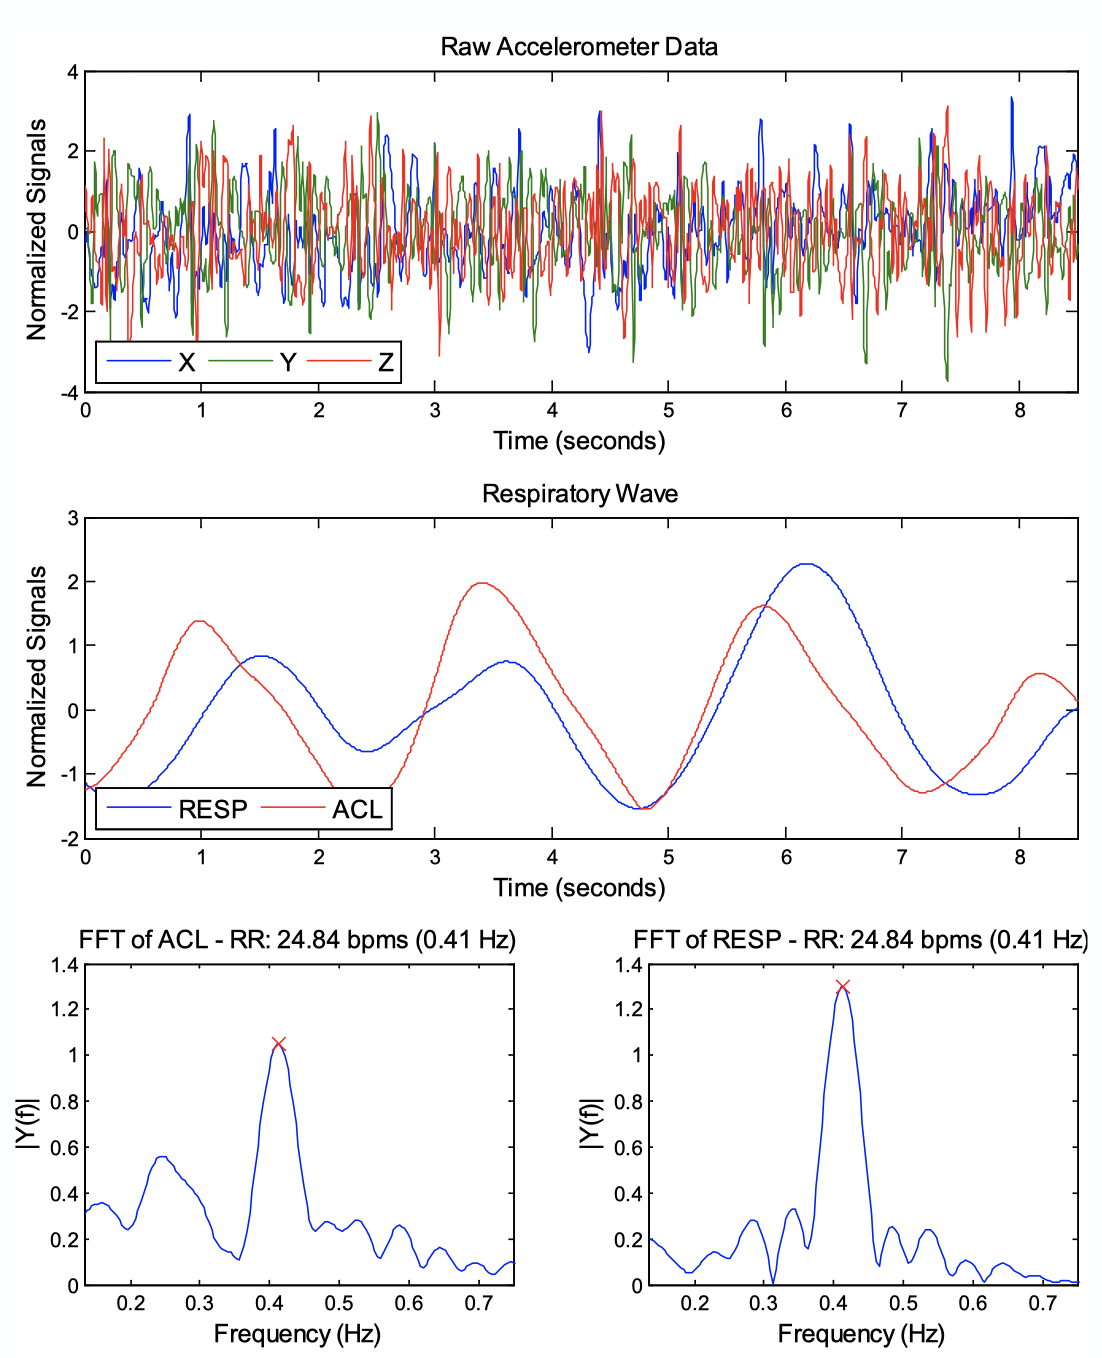
\includegraphics[width=\textwidth]{imu_research/googleGlass_respiratory_fig3}
      \caption{Beispiel einer Schätzung des Atemsignals anhand der Beschleunigungsdaten (blau) und des Ground-Truthsignals (rot). Die beiden unteren Graphen zeigen das Fourierspektrum von jedem Signal. (FFT: Fourier Spectrum, ACL: accelerometer, RESP: Respiration from chest band, RR: respiration rate, bpms: breaths per minute)}
      \label{background:googleGlass:respiratory_wave}
    \end{subfigure}
    \caption{Herzrate- und Atemfrequenzanalyse}
    \label{background:googleGlass}
  \end{figure}

Die Abbildung \ref{background:googleGlass:pulse_wave} zeigt ein Signal des Herzschlags, gesammelt von den Informationen der Gyroskopdaten. Diese Daten wurden mit der Google-Glass Brille aufgezeichnet, während die Person auf dem Rücken lag. Der obige Graph zeigt ein 3-Achsen Gyroskop signal über eine Dauer von 5.5 Sekunden. Der mittlere Graph zeigt die Schätzung des Herzschlags, nachdem die vorgestellten Methoden angewandt wurden in rot, die des Referenzsignals in blau. Es ist sehr gut zu erkennen, dass die Schätzung sehr nahe an den Referenzsignalen ist.

\subsubsection{Atemsignal}
Das Atemsignal wurde durch verschiedene Schritte berechnet:
\begin{itemize}
    \item Ein gleitender Mittelwertfilter wurde auf jede Komponente angewandt. Die Fensterlänge wurde auf die Dauer eines Atemzyklus gesetzt, in diesem Fall 45 Atmungen pro Minute. 
    \item Ein Bandpass Butterworthfilter der 4. Ordnung mit den Cut-Off Frequenzen von $0.13 \si{\hertz}$ und $0.75 \si{\hertz}$ (entspricht 8-45 Atmungen pro Minute) wurde auf jede Dimension angewandt.
    \item Da die verschiedenen Dimensionen der Sensoren nicht in Relation zu den Körperpositionen stehen, wurde eine Principal Component Analyse angewandt, um einen derartigen Einfluss zu reduzieren. Nach einer Fast Foiuriertransformation (FFT) auf jede Komponente wurde das Signal mit der Periode mit der maximalen Größenordnung ausgewählt, welche innerhalb des zu betrachtenden Frequenzbereichs liegt.
\end{itemize}

Die Abbildung \ref{background:googleGlass:respiratory_wave} zeigt ein Beispiel einer Atemfrequenzschätzung der Beschleunigungsdaten eines Patienten. Wie zu sehen ist, sind die Daten sehr nahe an dem Referenzwert, welcher mit aufgezeichnet wurde.


\subsection{Überwachung von Puls und Atmung mittels eSense-Earpods}
2019 wurde von \textit{Tobias Röddiger}, \textit{Daniel Wolffram} und \textit{David Laubenstein} nachgewiesen, dass es möglich ist, mittels den eSense-Earpods die Atmung und den Puls in Annäherung zu ermitteln \cite{roddigerRespirationRateMonitoring2019}. 
Dies gelang etwas genauer, als das Monitoring von \textit{J. Hernandez} mit dem Google Glass \cite{hernandezCardiacRespiratoryParameter}
Es wurden hierbei eine Studie mit 12 Personen aufgezeichnet, welche in 3 Positionen (liegend, stehend, sitzend) jeweils vor, beziehungsweise nach einer sportlichen Bewegungsphase einen einminütigen Atemablauf durchgeführt haben. 
Die Analyse der Daten erfolgte im Anschluss der Studie und wurde in einer Pipeline verarbeitet, welche zuerst das Rauschen reduziert, anschließend einen Triangle-Filter der Breite $2\si{\s}$ anwendet und danach eine PCA (engl. \textit{principal component analysis}) ausführt, um die Daten unabhängig von deren Achse zu bewerten.
Nun wurden Fenster mit der Größe von $20\si{\s}$ extrahiert, welche die Atmung und den Puls anhand dieses Fensters berechnen.
Die Resultate ergaben einen mittleren absoluten Fehler (engl. \textit{mean absolute error}) von 2.62 CPM (acc) und 2.55 CPM (gyro), jedoch variieren diese von Proband zu Proband.

Der Ablauf der Analyse beginnt damit, dass ein gleitendes Durchschnittsfenster (\textit{sliding average window}) von 3 Samples von jeder Dimension abgezogen wird. 
Zudem wird auf jeder der Komponenten ein Mittelwertfilter angewandt. 
Diese haben eine Fenstergröße von 2 Sekunden. 
Das soll Sinalverschiebungen und Signaltrends entfernen.
Anschließend wird eine kubische Splineinterpolation auf den Datensatz angewandt, um die Daten aufzublasen.
Falls zuviel Bewegung in einem Fenster zu erkennen ist, wird das Fenster verworfen \cite{sunSleepMonitorMonitoringRespiratory2017}.
Daraufhin wird ein Bandpass-Butterworth-Filter der 4. Ordnung auf den Datensatz angewandt, um das Rauschen zu entfernen.
Zum weiteren Glätten der Signale wird ein Dreiecksfilter angewandt \cite{haotianMindfulWatch2017}, worauf schließlich eine Hauptkomponentenanalyse (PCA) durchgeführt wird.
Auf jede Hauptkomponente wird nun eine Spektralanalyse mithilfe einer Fourier-Transformation (FFT) angewandt. 
Die Frequenz, welche dem Peak mit der höchsten Magnitude entspricht, resultiert schlussendlich als Atmungsfrequenz.

\begin{figure}[ht]
    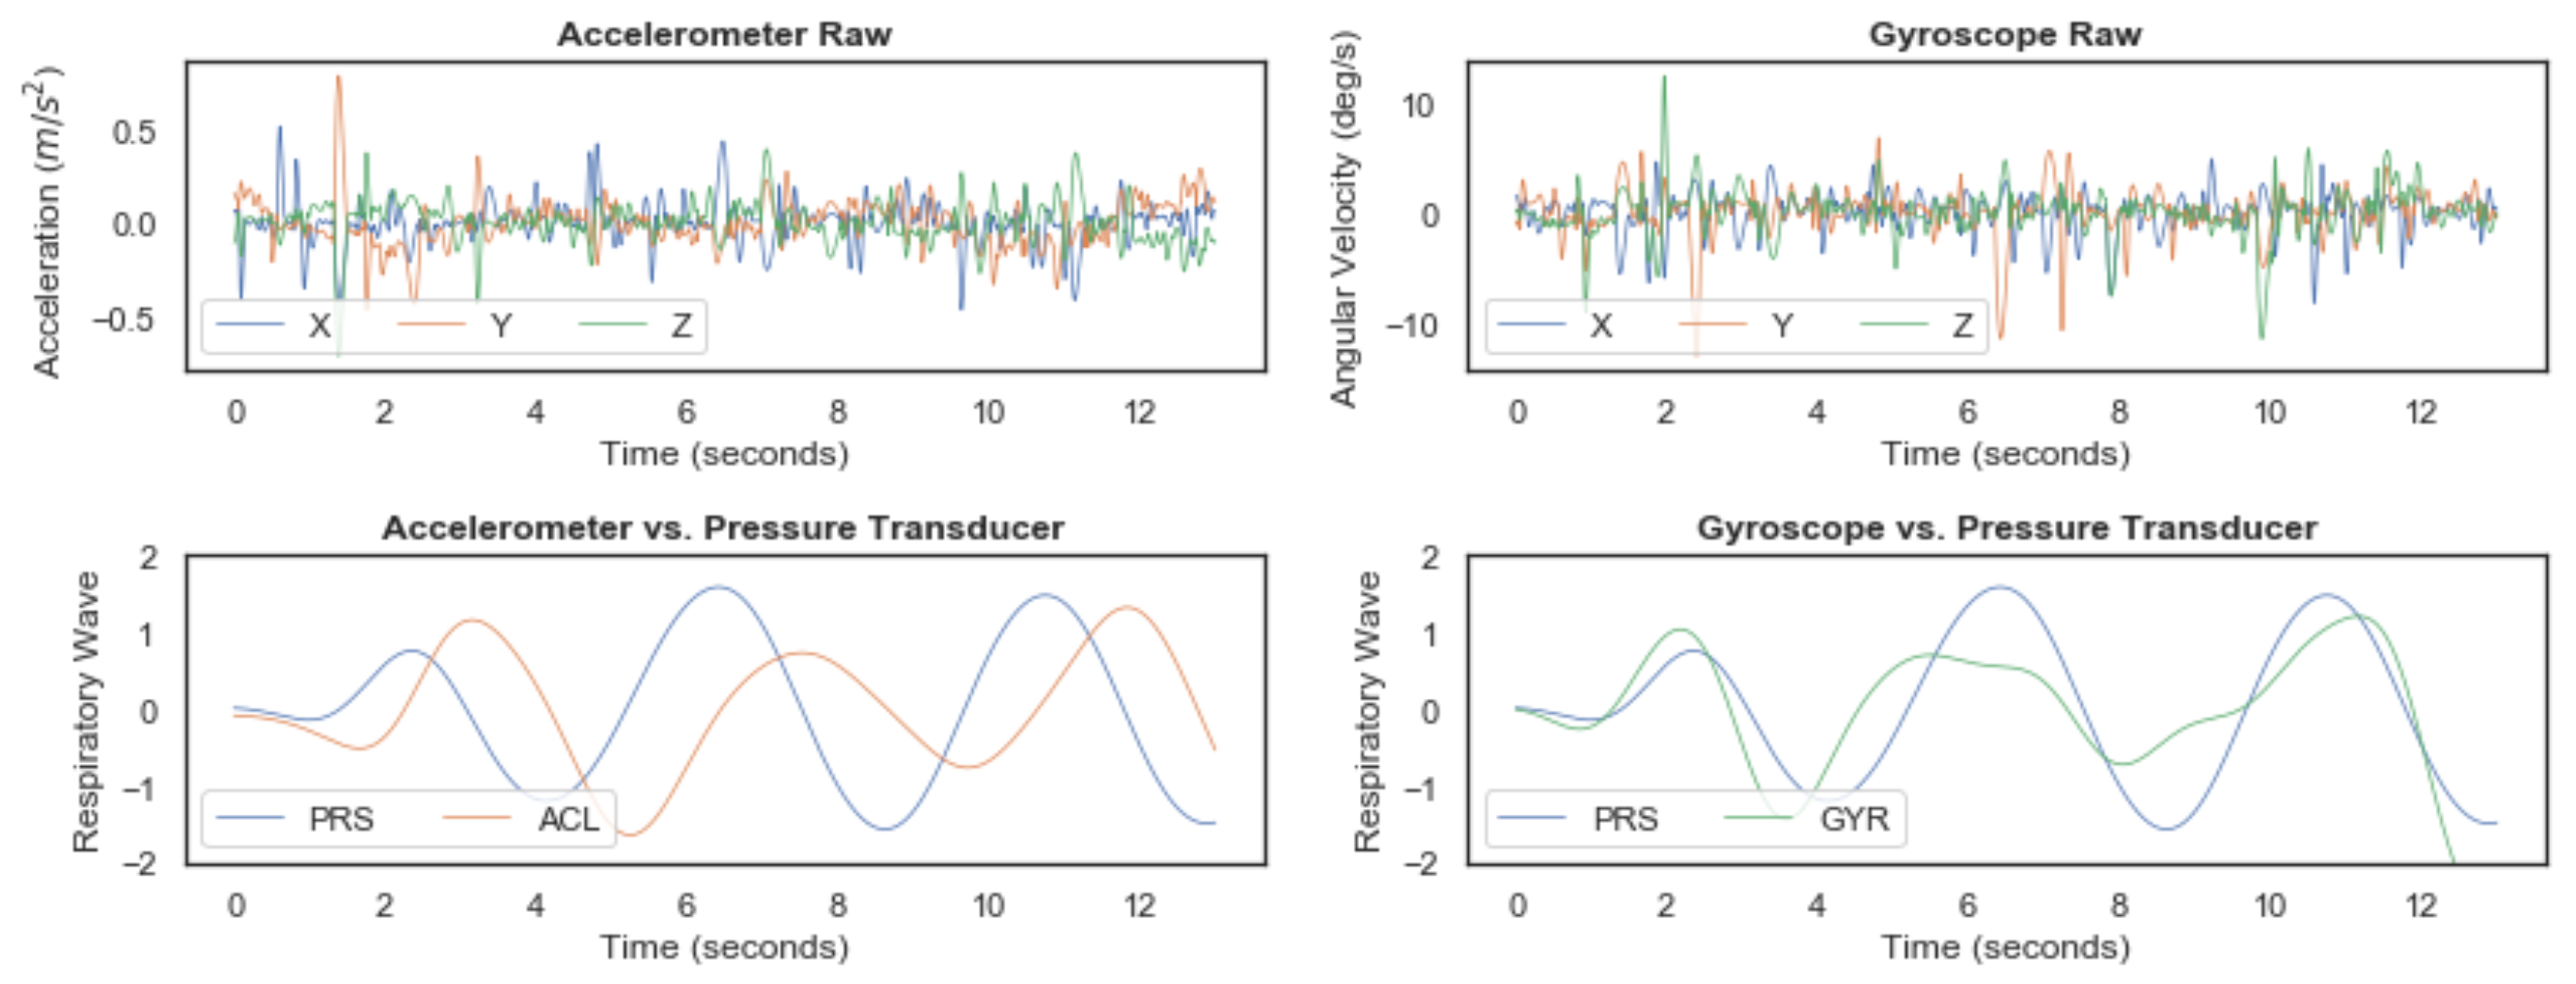
\includegraphics[width=1\textwidth]{imu_research/towards_resp_rates_waves}
    \caption{Rohdaten der Beschleunigungs- und Gyroskopdaten innerhalb von $12 \si{\s}$, sowie die Atem- und Pulsschätzung, verglichen mit dem Ground-Truh (blau)}
    \label{background:towards_resp_esense:results}
\end{figure}